\chapter{Energy Estimators}
\label{chap:MoreStuff}

\chapterquote{There, sir! that is the perfection of vessels!}
{Jules Verne, 1828--1905}

%========================================================================================
%========================================================================================

\section{Calibration}

%========================================================================================

\subsection{Calibration in the particle flow paradigm}
% Results use detector model 85 and calibration variant 71

\textcolor{red}{TODO: Trim down.}

In any experiment, calibration is essential for ensuring reliability in measured quantities and the linear collider will be no exception to this.  At the linear collider there will be several measured quantities each of which will be converted into a measure of the energy deposited in a given region of the detector.  These fall into two distinct classes (i) calorimeter energy deposits and (ii) track deposits.  The focus of this section will be on the energy deposits in the calorimeter and the procedure developed to ensure that they are reliable.  

Calorimeter energy deposits are an essential building blocks for the application of the particle flow paradigm.  The separation of energy deposits from charged and neutral particles in the calorimeters is crucial to achieve the full potential of particle flow and this is only possible with accurate energy estimators for those energy deposits.  A robust calibration scheme has been developed and will be discussed in the following chapter. 

The other crucial energy deposit used in particle flow calorimetry are track energy deposits.  These are also crucial to physics performance, however, in the particle flow paradigm these energy deposits are topologically related to the energy of the reconstructed particle.  A spatial helix fit is applied to the track energy deposits which when combined with knowledge of the magnetic filed yields the momentum of the particle producing the track.  Therefore, there is no direct relationship between the energy deposited by the monte-carlo particle in the active medium and the energy of the reconstructed energy.  Therefore, precise calibration of the energy deposited by a charged particle track is less crucial than for calorimeter energy deposits.  For this reason the focus of this chapter is on the calibration of calorimeter energy deposits. 

Calibration of the linear collider simulation extends beyond the raw calorimeter hits and into the particle flow algorithm itself.  The fine calorimeter granularity required for particle flow calorimetry yields excellent physical separation of hadronic and electromagnetic showers.  Thanks to sophisticated particle identification occurring within PandoraPFA it is possible to distinguish hadronic and electromagnetic showers, which allows for distinct treatments of the hadronic and electromagnetic energy estimators.  This distinction can be used to produce a response from the calorimeter that is compensating despite the intrinsic response being non-compensating.  A compensating calorimeter would give significant improvements to the energy resolution for the detector.

Two treatments designed to achieve a compensating response from the calorimeters are discussed.  The both involve rescaling the energies, the first rescaling is applied using a series of fixed energy independent constants, while the second uses the energy density of the calorimeter hits in the shower to determine the energy rescaling factor.

%========================================================================================

\subsection{Calibration and detector optimisation}
Optimising the detector at a future linear collider will be crucial to exploit the full physics potential available to it.  An extensive optimisation of the calorimeters was performed and the results can be found in chapter \ref{sec:optimisationstudies}.  For each detector model considered in this study the calibration procedure outlined in this section was applied to ensure optimal performance was achieved.  This made unbiased comparison between detector models performance possible and ensured reliability in the conclusions drawn from this study.

%========================================================================================

\subsection{Calibration Goals}
The calibration procedure aims to accurately set parameters related to four aspects of the reconstruction, which are:

\begin{enumerate}
\item \textbf{Digitisation of calorimeter hits}.  Digitisation in this sense is the estimation of the energy deposited within a calorimeter cell, the active and absorber layers, based on the signal measured in the sensitive region of the cell, the active layer.  
\item \textbf{Minimum ionising particle (MIP) scale setting in the digitisation processor and PandoraPFA}.  The MIP scale has to be set in the digitiser as it simulates the response of the readout technology including a maximum readout value, which is in units of MIPs, while PandoraPFA uses the MIP scale to place cuts to veto noise from the detector.  While no noise is applied to the simulation these cuts are still applied to better represent the performance of PandoraPFA using real data.  
\item \textbf{Electromagnetic and hadronic scale setting in PandoraPFA}.  As discussed in chapter CALORIMETER CHAPTER, the response of a calorimeter to electromagnetic and hadronic showers is different due to the fundamentally different mechanisms governing their propagation.  One key difference between the two is the presence of an invisible energy component in the hadronic shower.  Therefore, the reported energy from a calorimeter to a hadronic showers will be lower than that of an electromagnetic shower.  To account for effects such as this and to account for energy losses due to the application of noise vetoing cuts in PandoraPFA the PFO energies are rescaled by PandoraPFA depending on whether the PFO has showered electromagnetically or hadronically.  Determination of these scaling factors is the setting of the electromagnetic and hadronic energy scales.  
\item \textbf{Retraining photon likelihood data}.  The PandoraPFA algorithm uses likelihood data to determine whether a reconstructed object is a photon.  This likelihood data has to be retrained for every new detector model considered. 
\end{enumerate}

Each of these aspects needs separately addressing for each new detector model considered.  The ordering of each of these calibration steps also had to be taken into consideration as it is possible to get interference between the different stages if applied in the wrong order.  

%========================================================================================

\subsection{Digitisation}
Calibration of the digitisation of the calorimeter hits involves accurately estimating the energy deposited in a calorimeter cell, in both the active and absorber layers, based on the energy deposited in the sensitive element of the calorimeter, the active layer.  The relationship between the energy deposited in the active layers and the absorber layers of a calorimeter is linear as the energy deposited in both layers are proportional to the number of charged tracks passing through them.  The ratio of the calorimeter cell energy to the energy deposited in the active layers is hereby called the digitisation constant.  
.
The digitisation constants depend upon several aspects of the detector including the material properties of the calorimeters, the magnetic field strength and energy losses occurring within the gaps between the active and absorber layers.  To account the effect of instrumented read out technology that would exist in a completed calorimeter some material is included in the simulation around the active and absorber layer.  In comparison to the absorber layer this extra material adds little to the detector, but energy losses here are accounted for in digitisation.  

%========================================================================================

\subsubsection{ECal Digitisation}
The procedure for determining the digitisation constants in the ECal involved the simulation of single $\gamma$ events at $E_{MC} = 10$ GeV.  $\gamma$ events are ideal for calibration of the ECal as in the particle flow paradigm $\gamma$ energy measurements are made primarily within the ECal.  Also at this energy $\gamma$s are largely contained within the ECal, as shown in figure \ref{fig:ecaldigiphotonsplit}, making them ideal for isolating the ECal digitisation calibration from that of the HCal digitisation calibration.   

\begin{figure}
  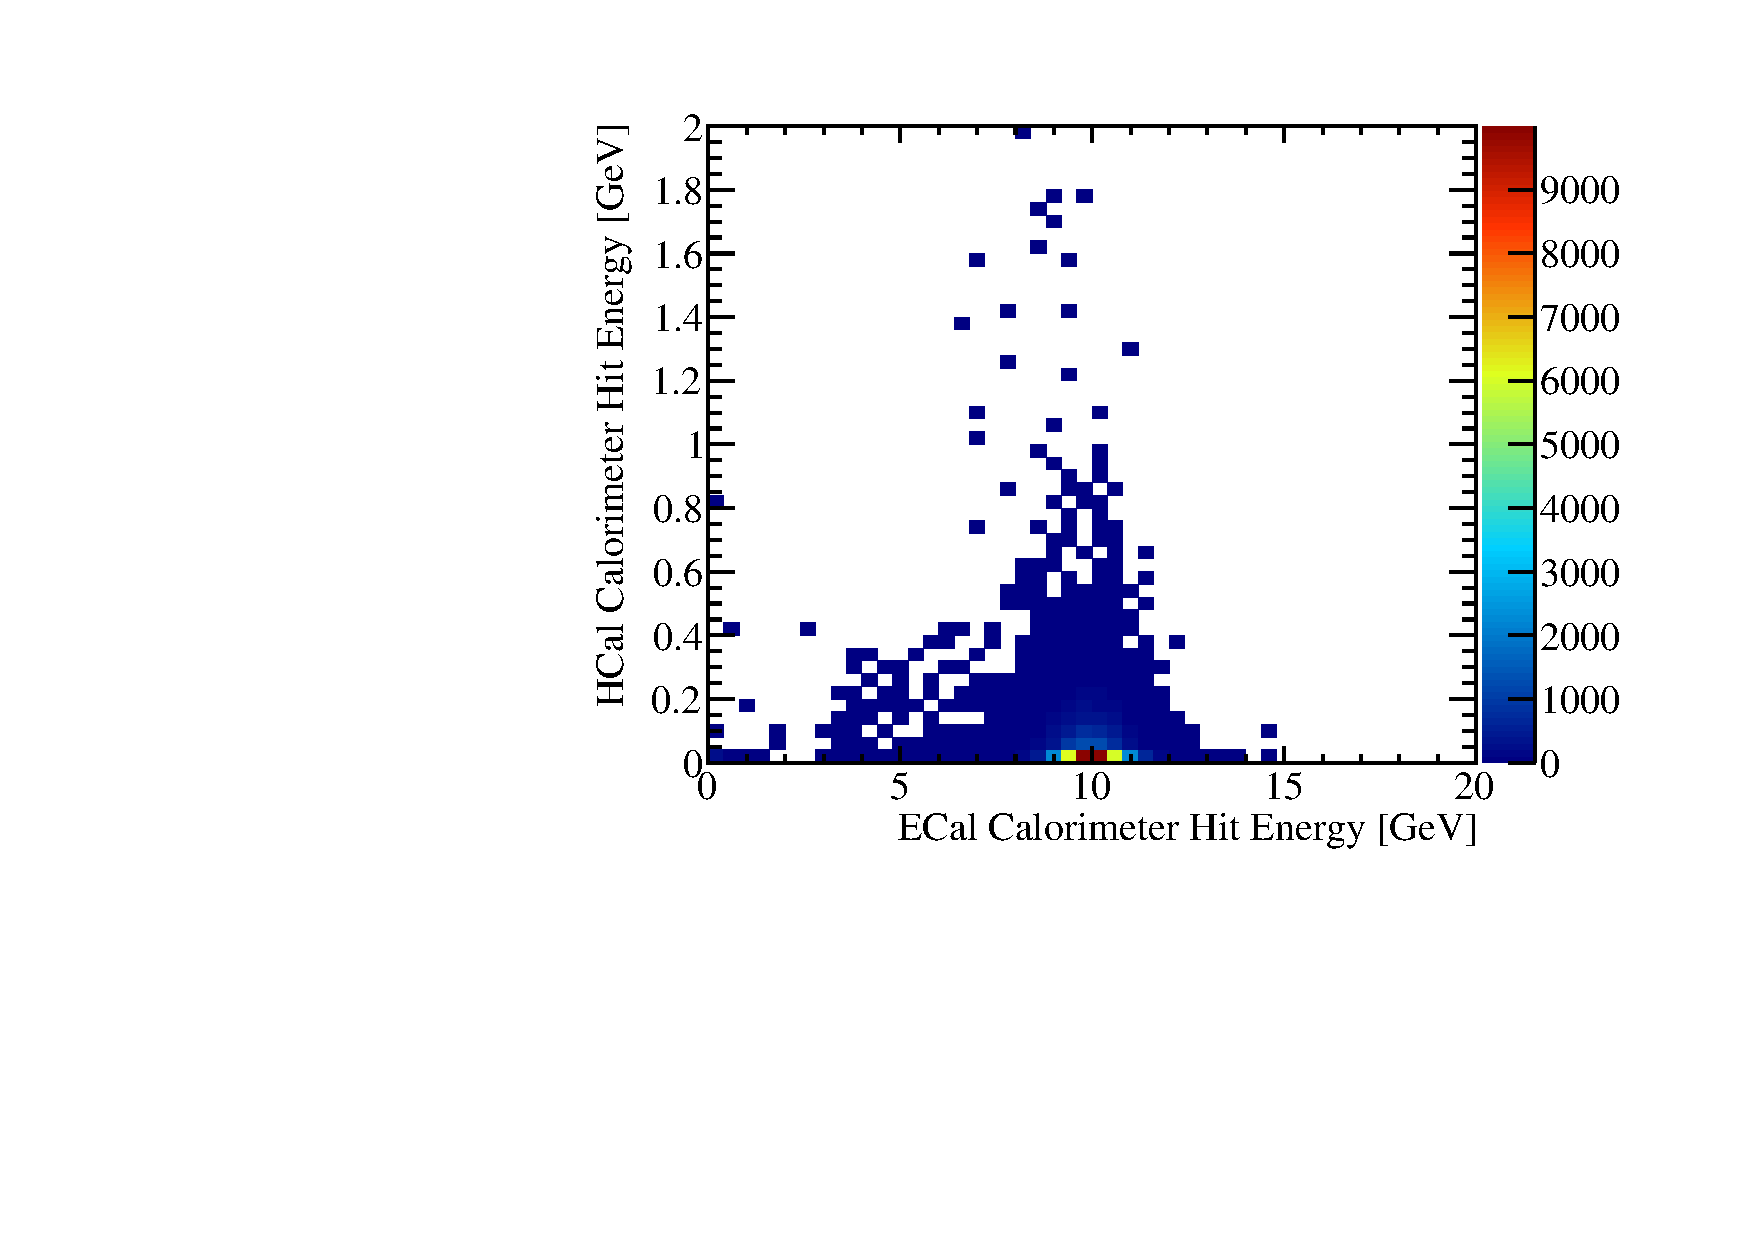
\includegraphics[width=\largefigwidth]{EnergyEstimators/Plots/Calibration/Digitsation/ECal/ECalHCalPhotonSplit.pdf}
  \caption[Sum of calorimeter hit energies in ECal and HCal for 10 GeV $\gamma$ events.]{Sum of calorimeter hit energies in ECal and HCal for 10 GeV $\gamma$ events.}
  \label{fig:ecaldigiphotonsplit}
\end{figure}

Events are only considered in this analysis if they are confined to the ECal and to that extent cuts are applied ensuring that the sum of any reconstructed energy found outside the ECal is less than 1\% of $E_{MC}$ and that the $\text{cos}(\theta) < 0.95$ where $\theta$ is the polar angle of the $\gamma$.  $\gamma$ conversions are also vetoed from this event sample at this stage.  The impact of these cuts on the sum of ECal calorimeter hit energies for the $E_{MC} = 10$ GeV $\gamma$ events is shown in figure \ref{fig:ecaldigiselection}.

\begin{figure}
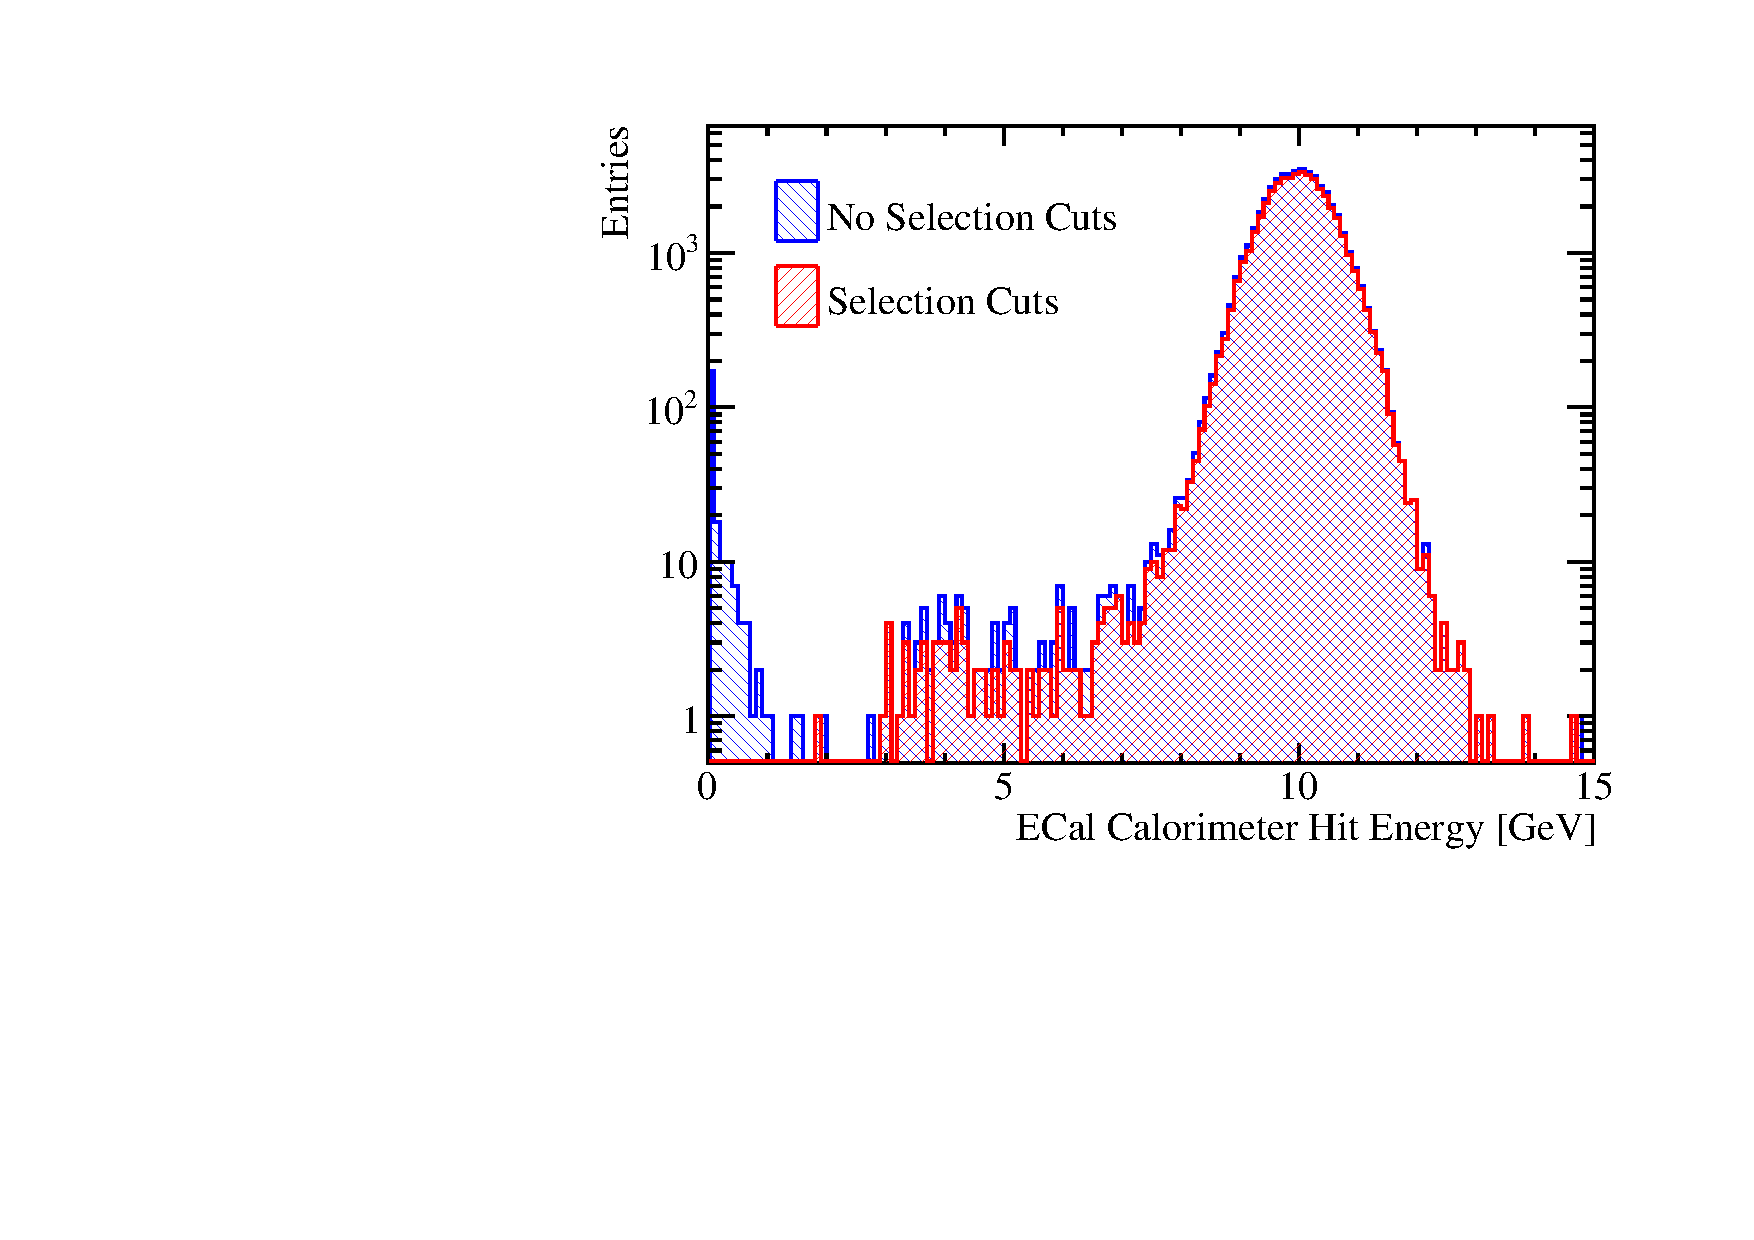
\includegraphics[width=\largefigwidth]{EnergyEstimators/Plots/Calibration/Digitsation/ECal/DigitisationECalSelection.pdf}
\caption[Sum of the ECal calorimeter hit energies for a 10 GeV photon with and without the selection cuts.]{Sum of the ECal calorimeter hit energies for a 10 GeV photon with and without the selection cuts.}
\label{fig:ecaldigiselection}
\end{figure}

\begin{figure}
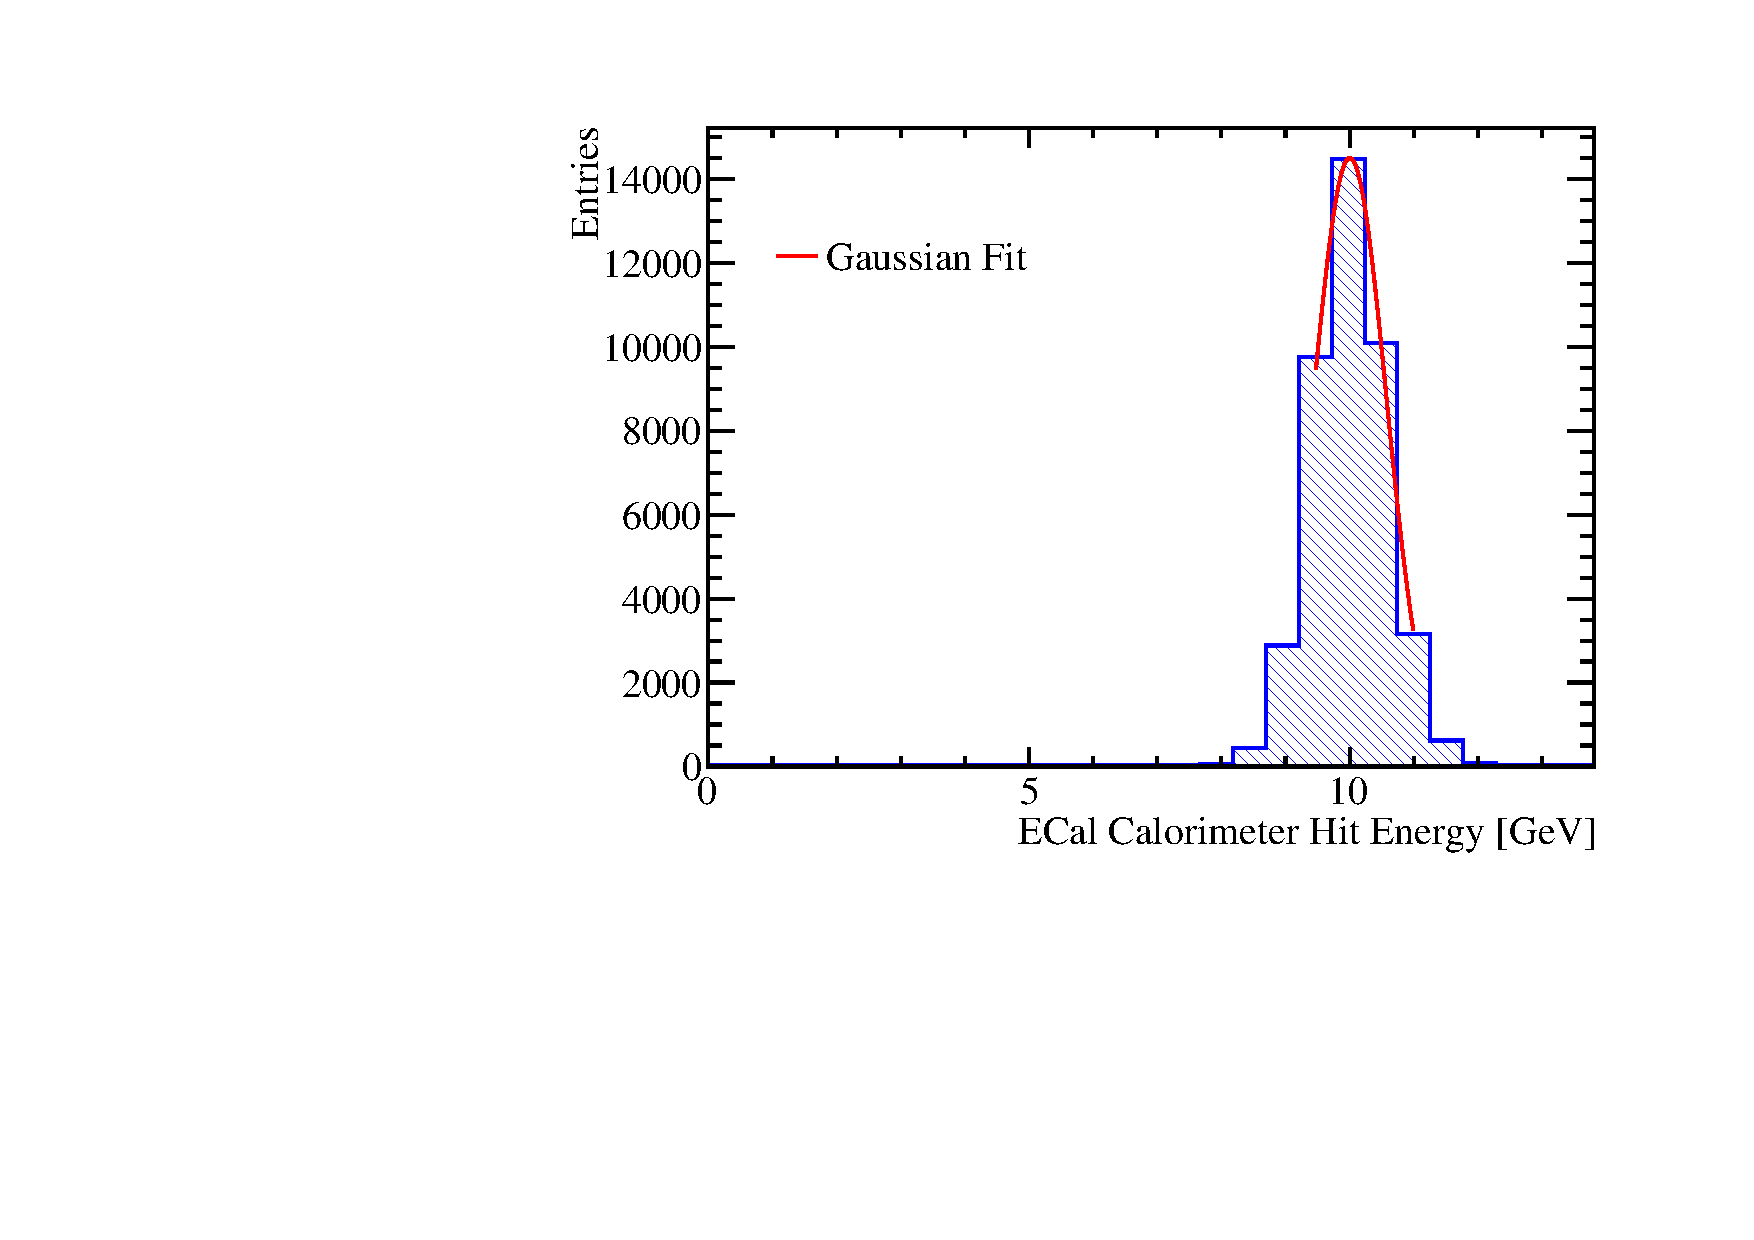
\includegraphics[width=\largefigwidth]{EnergyEstimators/Plots/Calibration/Digitsation/ECal/DigitisationECalFit.pdf}
\caption[Gaussian fit to sum of the ECal calorimeter hit energies for a 10 GeV photon with selection cuts.]{Gaussian fit to sum of the ECal calorimeter hit energies for a 10 GeV photon with selection cuts.}
\label{fig:ecaldigifit}
\end{figure}

The calibration procedure is iterative and begins with the simulated single $\gamma$ events using a trial calibration, with digitisation constant in the ECal $\alpha^{0}_{\text{ECal}}$, which may not be ideal.  Then the distribution of the sum of calorimeter hit energies within the ECal is produced for events passing the selection cuts using, as shown in figure \ref{fig:ecaldigiselection}.  For an ideal calorimeter this distribution should be Gaussian, as was described in section CALORIMETER CHAPTER.  Therefore, a Gaussian fit is applied to this distribution and the mean, $E_{\text{Fit}}$, extracted.  In an attempt to remove the effect of any outliers in this distribution, the fit is applied to the range of data with the smallest root mean square that contains at least 90 \% of the data.  An example of such a fit is shown in figure \ref{ig:ecaldigifit}.  In the case of perfect calibration the mean of this fit would be equal $E_{MC}$ and it is assumed that any deviation between the two is due to inaccurate calibration.  To correct for any such deviation the digitisation constant from the trial calibration, $\alpha^{0}_{\text{ECal}}$, is rescaled by the ratio of the $E_{MC}$ to $E_{\text{Fit}}$.

\begin{equation}
\alpha^{0}_{\text{ECal}} \rightarrow \alpha_{\text{ECal}} = \alpha^{0}_{\text{ECal}} \times \frac{E_{MC}}{E_{Fit}}
\end{equation}

This procedure is then repeated until the $E_{\text{Fit}}$ falls within a chosen tolerance of $E_{\text{MC}}$.  The tolerance that was applied here is that $|E_{\text{Fit}} - E_{\text{MC}}| < E_{\text{MC}} \times 5 \%$.  The binning for the fitted histogram is chosen such that the bin width is equal to the desired tolerance on $E_{\text{Fit}}$ e.g. $E_{\text{MC}} \times 5 \% = 0.5$ GeV.  This tolerance is somewhat large, however, it is tight enough to ensure successful application of PFA.  It should also be emphasised that the PFO energies used in downstream analyses have the electromagnetic and hadronic energy scale corrections applied and these are  calibrated to a much tighter accuracy.

\subsubsection{HCal Digitisation}

%========================================================================================

\subsection{MIP Scale Setting}

%========================================================================================

\subsection{Electromagnetic and hadronic scale setting}

%========================================================================================



\begin{figure}
  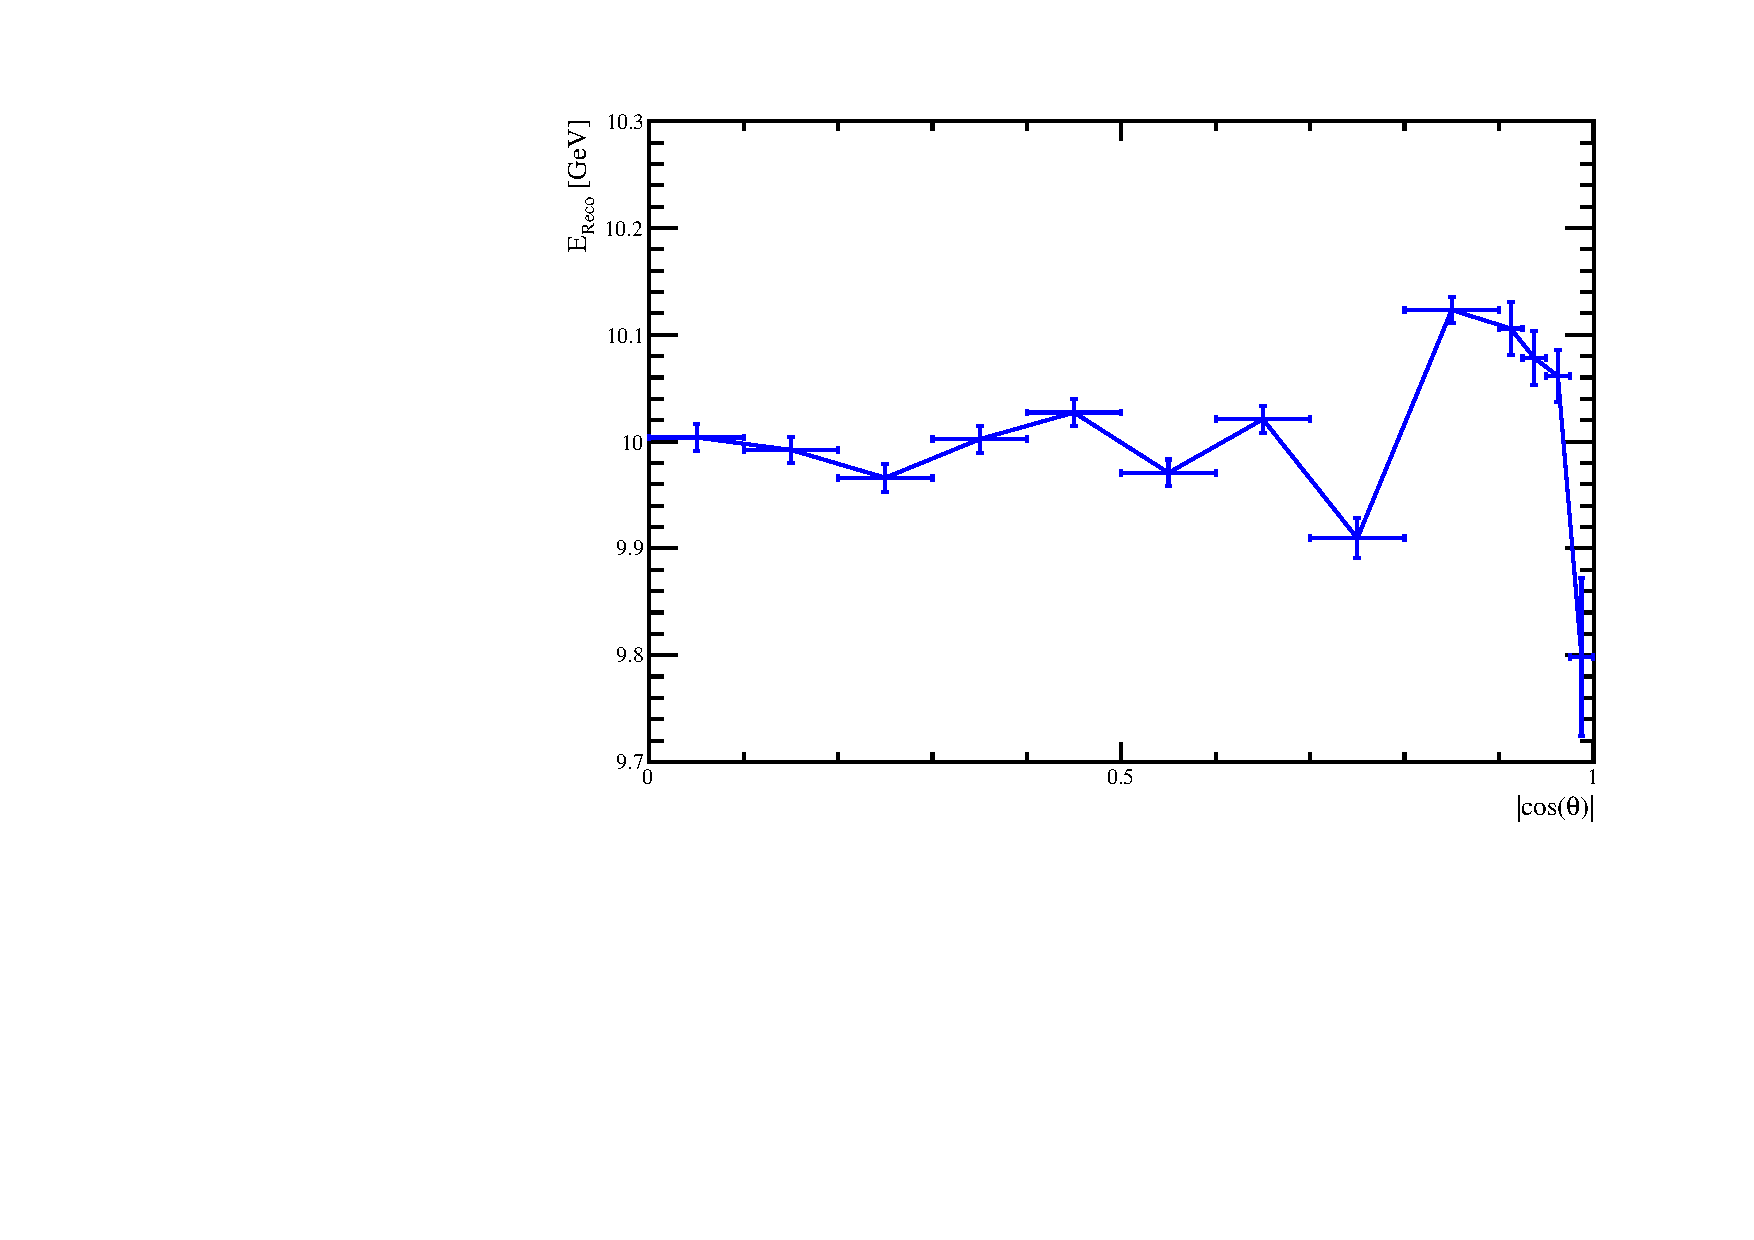
\includegraphics[width=\largefigwidth]{EnergyEstimators/Plots/Calibration/Validation/AngularDistributionPhotonPlot.pdf}
  \caption[Mean reconstructed photon energy as a function of the polar angle of the photon.]{Mean reconstructed photon energy as a function of the polar angle of the photon.}
  \label{engest:fig:photonangle}
\end{figure}

\begin{figure}
  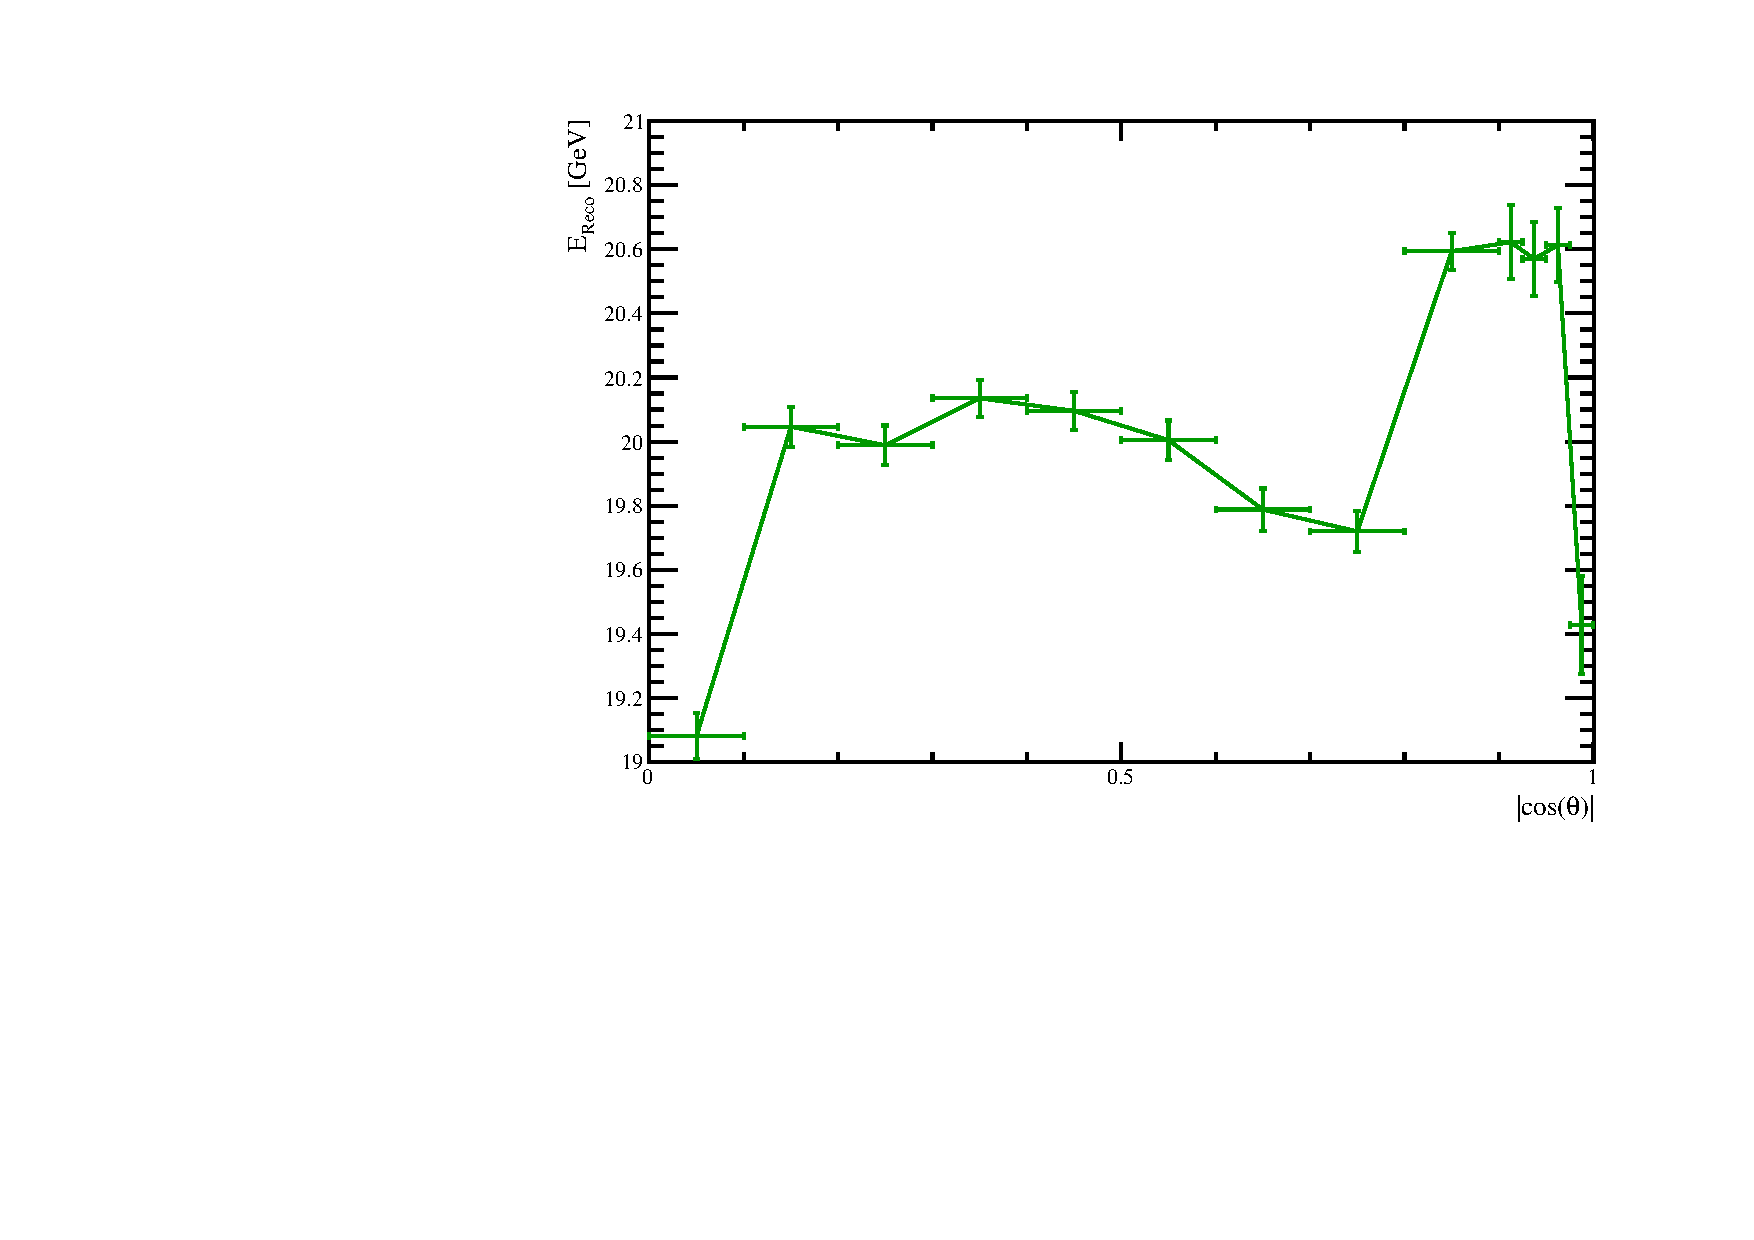
\includegraphics[width=\largefigwidth]{EnergyEstimators/Plots/Calibration/Validation/AngularDistributionKaon0LPlot.pdf}  \caption[Mean reconstructed kaon0L energy as a function of the polar angle of the kaon0L.]{Mean reconstructed kaon0L energy as a function of the polar angle of the kaon0L.}
    \label{engest:fig:photonangle}
    \end{figure}


\iffalse
Validation 
/Users/stevengreen/Thesis/EnergyEstimators/Plots/Calibration/Validation
207:Validation stevengreen
AngularDistributionKaon0LPlot.pdf AngularDistributionPhotonPlot.pdf

SoftComp
/Users/stevengreen/Thesis/EnergyEstimators/Plots/SoftComp/DrawWeights.C /Users/stevengreen/Thesis/EnergyEstimators/Plots/SoftComp/MakePlots.C /Users/stevengreen/Thesis/EnergyEstimators/Plots/SoftComp/PfoEnergyKaon0L.C /Users/stevengreen/Thesis/EnergyEstimators/Plots/SoftComp/PFOEnergySoftComp.pdf /Users/stevengreen/Thesis/EnergyEstimators/Plots/SoftComp/Weights.C 

Calibration
/Users/stevengreen/Thesis/EnergyEstimators/Plots/Calibration/Calorimeter_Hit_Energies_ECal_Digitisation.C /Users/stevengreen/Thesis/EnergyEstimators/Plots/Calibration/Calorimeter_Hit_Energies_HCal_Barrel_Digitisation.C /Users/stevengreen/Thesis/EnergyEstimators/Plots/Calibration/Calorimeter_Hit_Energies_HCal_EndCap_Digitisation.C /Users/stevengreen/Thesis/EnergyEstimators/Plots/Calibration/Direction_Corrected_SimCalorimeterHit_Energy_Distribution_ECal_10_GeV_Muons.C /Users/stevengreen/Thesis/EnergyEstimators/Plots/Calibration/Direction_Corrected_SimCalorimeterHit_Energy_Distribution_HCal_10_GeV_Muons.C /Users/stevengreen/Thesis/EnergyEstimators/Plots/Calibration/Direction_Correction_Distribution_HCal_20_GeV_KaonL.C /Users/stevengreen/Thesis/EnergyEstimators/Plots/Calibration/ECalDigitsation.pdf /Users/stevengreen/Thesis/EnergyEstimators/Plots/Calibration/EMPandora.pdf /Users/stevengreen/Thesis/EnergyEstimators/Plots/Calibration/GeVToMIP_Calibration_10_GeV_Muons_ECal.C /Users/stevengreen/Thesis/EnergyEstimators/Plots/Calibration/GeVToMIP_Calibration_10_GeV_Muons_HCal.C /Users/stevengreen/Thesis/EnergyEstimators/Plots/Calibration/GeVToMIP_Calibration_10_GeV_Muons_Muon_Chamber.C /Users/stevengreen/Thesis/EnergyEstimators/Plots/Calibration/HadPandora.pdf /Users/stevengreen/Thesis/EnergyEstimators/Plots/Calibration/HCalDigi.pdf /Users/stevengreen/Thesis/EnergyEstimators/Plots/Calibration/MIPResponseECalDigi.pdf /Users/stevengreen/Thesis/EnergyEstimators/Plots/Calibration/MIPScalePandora.pdf /Users/stevengreen/Thesis/EnergyEstimators/Plots/Calibration/PandoraPFA_Calibration_Electromagnetic_Energy_Scale_10_GeV_Photons.C /Users/stevengreen/Thesis/EnergyEstimators/Plots/Calibration/PandoraPFA_Calibration_Hadronic_Energy_Scale_Chi_Sqaured_Method_20_GeV_KaonL.C 
\fi


